\documentclass{article}
\usepackage[utf8]{inputenc}
\usepackage{amsmath}
\usepackage{graphicx}
\graphicspath{ {images/} }

\begin{document}

\section{Direkt geometria}
\subsection{Transzformációs mátrixok}
A quadruped középpontját origónak tekintve, ahol X irány jobbra, Y fölfele és Z előre mutat, a robot egy lábának csuklóinak és merev részeinek transzformációs mátrixai:

$$
\begin{pmatrix}
	1&0&0&d_x\\
	0&1&0&d_y\\
	0&0&1&d_z\\
	0&0&0&1
\end{pmatrix}	
\begin{pmatrix}
	C_1&0&S_1&0\\
	0&1&0&0\\
	-S_1&0&C_1&0\\
	0&0&0&1
\end{pmatrix}	
\begin{pmatrix}
	1&0&0&0\\
	0&1&0&0\\
	0&0&1&d_1\\
	0&0&0&1
\end{pmatrix}	
\begin{pmatrix}
	1&0&0&0\\
	0&C_2&-S_2&0\\
	0&S_2&C_2&0\\
	0&0&0&1
\end{pmatrix}
$$
$$
\begin{pmatrix}
	1&0&0&0\\
	0&1&0&0\\
	0&0&1&d_2\\
	0&0&0&1
\end{pmatrix}	
\begin{pmatrix}
	1&0&0&0\\
	0&C_3&-S_3&0\\
	0&S_3&C_3&0\\
	0&0&0&1
\end{pmatrix}	
\begin{pmatrix}
	1&0&0&d_{3x}\\
	0&1&0&0\\
	0&0&1&d_3\\
	0&0&0&1
\end{pmatrix}
$$
\subsection{Paraméterek}
Paraméterek értéke radiánban ill. mm-ben:\\\\
\begin{tabular}{ | l | l | l | l | l | l | l | l | l | l | l | }
	\hline
	láb&$\alpha_1$&$\alpha_2$&$\alpha_3$&$d_x$&$d_y$&$d_z$&$d_1$&$d_2$&$d_3$&$d_3x$\\
	\hline
	jobb első&$\pi/4$&$0$&$\pi/4$&$35$&$21$&$40$&$18$&$40$&$80$&$4$\\
	\hline
	jobb hátsó&$3\pi/4$&$0$&$\pi/4$&$35$&$21$&$-40$&$18$&$40$&$80$&$-4$\\
	\hline
	bal első&$-\pi/4$&$0$&$\pi/4$&$-35$&$21$&$40$&$18$&$40$&$80$&$-4$\\
	\hline
	bal hátsó&$-3\pi/4$&$0$&$\pi/4$&$-35$&$21$&$-40$&$18$&$40$&$80$&$4$\\
	\hline
\end{tabular}\\\\
Az $\alpha_n$ értékek az elfordulás offsetét jelzik. Ezek jelentősége, hogy a megvalósításnál alkalmazott motorok $-\pi$ és $\pi$ között tudnak mozogni, és ilyen offsetek mellett tud a robot lába legkényelmesebben pozíciókba állni.\\
A $d_x$, $d_y$ és $d_z$ az első motor tengelyébe való eltolás a második motor tengelyének magasságában,	$d_1$ az első és második, $d_2$ a második és utolsó motor tengelye közti eltolás, $d_3$ az utolsó motor tengelye és a láb vége közti eltolás, $d_{3x}$ pedig a láb vége és első motor tengelye közti oldalirányú eltolás, aminek iránya egybeesik a második és harmadik tengelyek irányával, így az első motor után mindegy hol vesszük figyelembe. A paraméterek jobban láthatóak a \ref{fig:param} képen.
\begin{figure}
	\caption{Lábak paraméterei}
	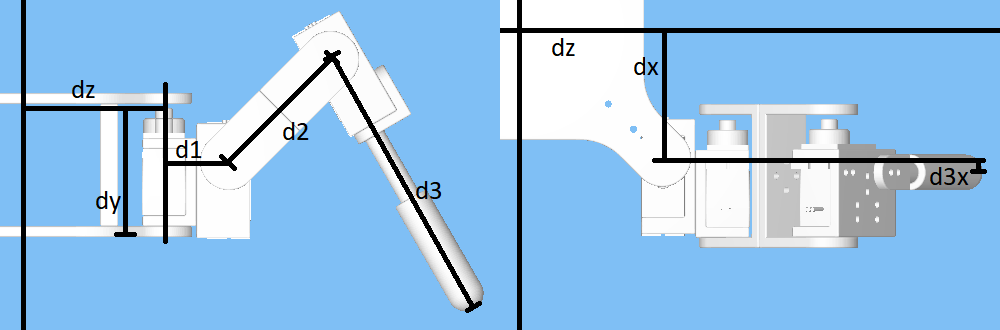
\includegraphics[width=\textwidth]{quad_params}
	\label{fig:param}
\end{figure}

\subsection{Számolás}
A transformációs mátrixokat összeszorozva egy láb rotaciós mátrixa és pozícióvektora:
$$
\begin{pmatrix}
C_1&S_1S_{23}&S_1C_{23}\\
0&C_{23}&-S_{23}\\
-S_1&C_1S_{23}&C_1C_{23}
\end{pmatrix}
=
Rot
$$
$$
\begin{pmatrix}
C_1d_3x+S_1C_{23}d_3+S_1C_2d_2+S_1d_1+d_x\\
-S_{23}d_3-S_2d_2+d_y\\
-S_1d_{3x}+C_1C_{23}D_3+C_1C_2d_2+C_1d_1+d_z
\end{pmatrix}
=
\begin{pmatrix}
p_x\\
p_y\\
p_z
\end{pmatrix}
$$
\\
A rotációs mátrix nem szükséges, a cél, hogy a láb vége az általunk mondott pozícióba kerüljön. Habár arra oda kell figyelni, hogy a lábfej ne alulról érintse a talajt, ami fizikailag lehetetlen. A megvalósításból adódóan ez csak akkor lenne lehetséges, ha az egész robot a talaj alatt lenne.


\end{document}
